\documentclass[12pt]{amsart}

\usepackage{amssymb}

\usepackage[letterpaper, margin=1in]{geometry}

\usepackage[final]{graphicx}


\begin{document}

\title{Your Title Here}

\author{Your Name}

\date{\today}

\maketitle

\section{Introduction}  PUT CONTENT HERE; PERHAPS CITE SOMETHING \cite{einstein}

%\begin{figure}
%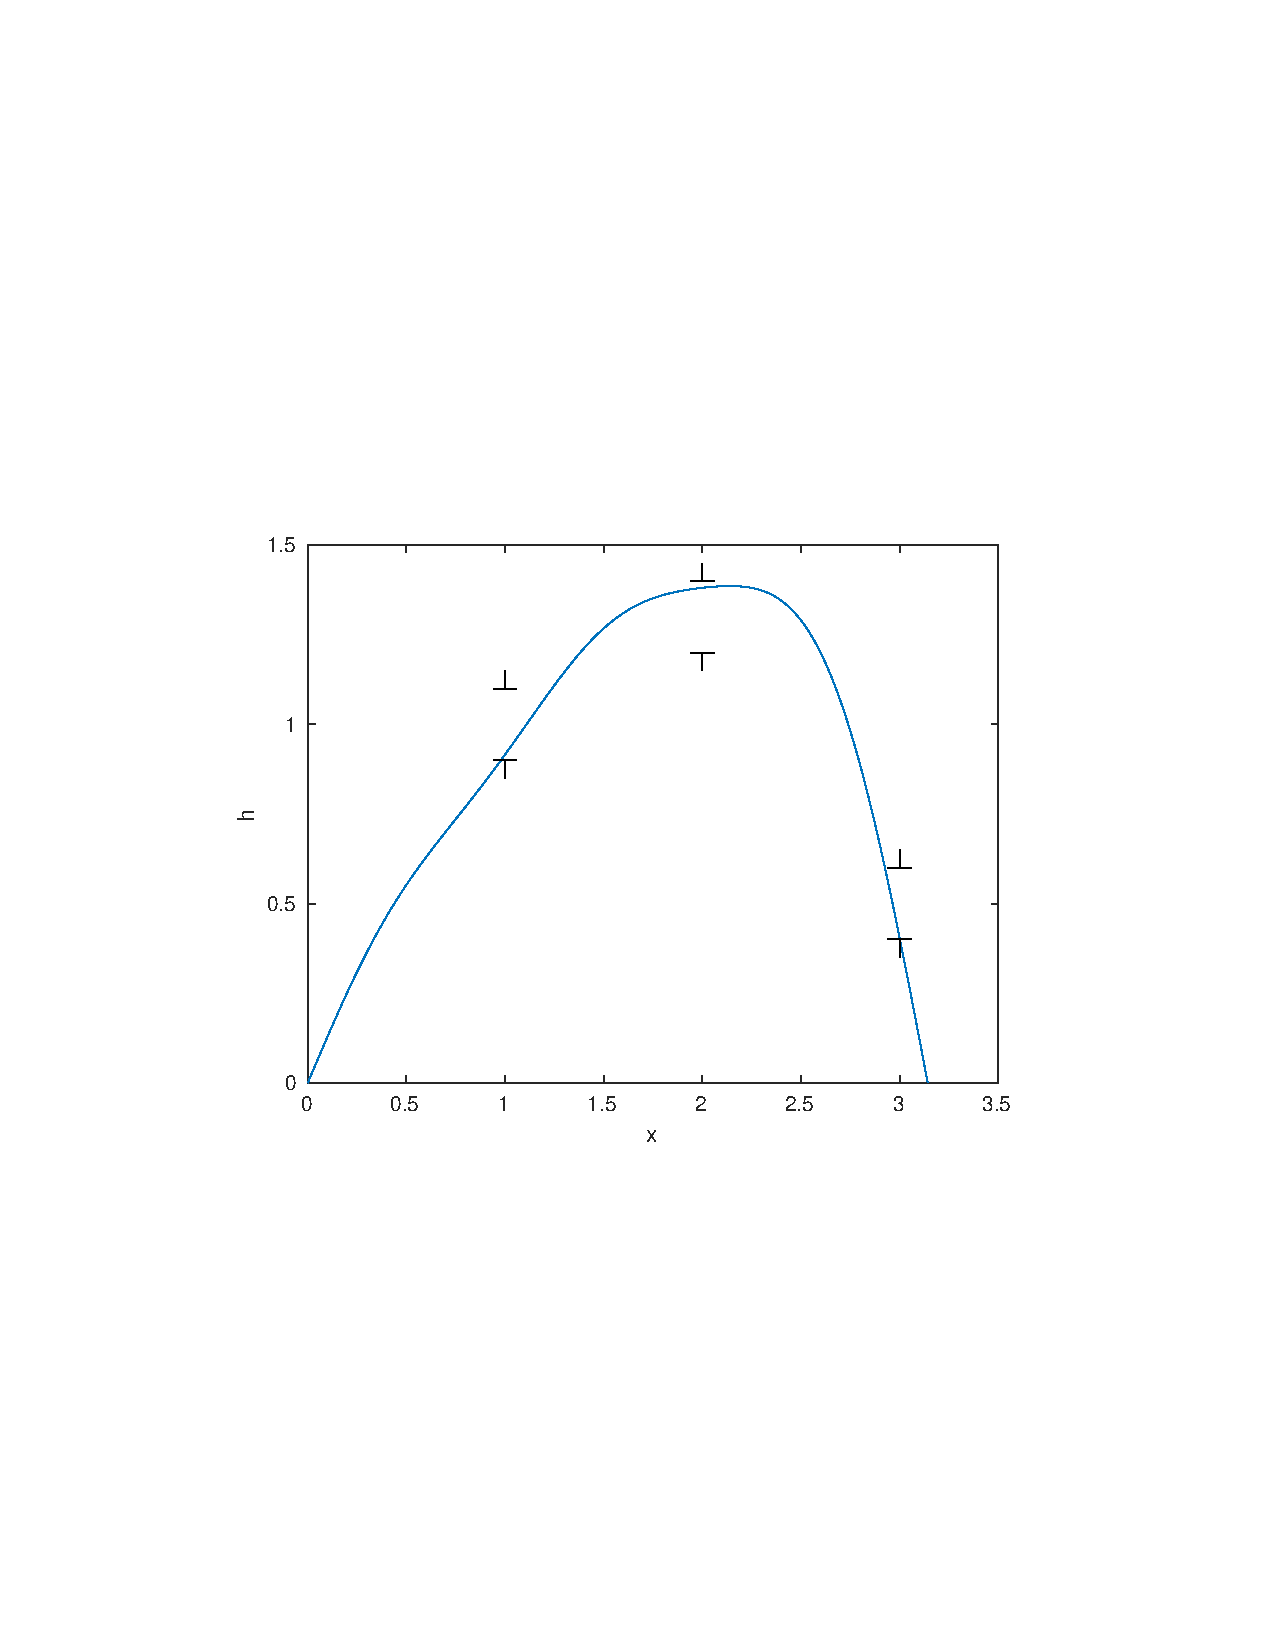
\includegraphics[width=0.5\textwidth]{foo.png}  % put image "foo.png" in current directory
%\caption{CAPTION TEXT HERE}
%\end{figure}

\section{Algorithms [or Examples]}  PUT CONTENT HERE; PERHAPS CITE SOMETHING \cite{nocedalwright}

\section{Examples [or Algorithms]}  PUT CONTENT HERE

\section{Implementation}  PUT CONTENT HERE

\bigskip
\hrule
\begin{verbatim}
% MYCODE  This is my matlab implementation
x = 1:10;
y = randn(size(x));
plot(x,y)
z = 2+2
\end{verbatim}
\hrule
\bigskip

MORE CONTENT PERHAPS

\bigskip
\hrule
\begin{verbatim}
>> mycode             % here I am running the code
z = 4
\end{verbatim}
\hrule

\section{Results}  PUT CONTENT HERE

\section{Analysis}  PUT CONTENT HERE

\section{Conclusion}  PUT CONTENT HERE

\begin{thebibliography}{2}  % "2" because there are two references
\bibitem{einstein} 
A.~Einstein (1905). 
\textit{Zur Elektrodynamik bewegter K{\"o}rper},
Annalen der Physik, 322 (10), 891--921.

\bibitem{nocedalwright}
J.~Nocedal \& S.~Wright (2006).
\textit{Numerical Optimization},
2nd ed., Springer.
\end{thebibliography}

\end{document}
